\documentclass[xcolor=dvipsnames]{beamer}

\usepackage[utf8]{inputenc}
\usepackage{multicol}
\usepackage{amssymb,amsmath,amsbsy,cmath} 
\usepackage{bm}    
\usepackage{graphicx,graphics,xcolor}
\usepackage{xcolor}
\usepackage{physics}
\usepackage{comment}
\usepackage{caption}
\usepackage[style=authortitle,backend=bibtex]{biblatex}
\addbibresource{References.bib}
\usepackage{yfonts}
\usepackage{pifont}


\newcommand\blfootnote[1]{%
  \begingroup
  \renewcommand\thefootnote{}\footcite{#1}%
  \addtocounter{footnote}{-1}%
  \endgroup
}
\newcommand{\RomanNumeralCaps}[1] {\MakeUppercase{\romannumeral #1}}

\usetheme{Madrid}
\useoutertheme{miniframes} % Alternatively: miniframes, infolines, split
\useinnertheme{circles}


\title[Schwarzschild geometry]{Schwarzschild Geometry: Static Black Holes}
\date{\today}
\author[Universidad del Valle]{Stiven Londoño}
\institute[]{Universidad del Valle \\ Departamento de física}

\begin{document}
	
	\begin{frame}
		\titlepage
	\end{frame}
	
	\begin{frame}{Table of contents}
    \tableofcontents
	\end{frame}
	
	
\section{Schwarzschild geometry}

\begin{frame}{Schwarzschild metric}
Consider a body of mass $M$ and let $\mu = GM/c^2$, then the Schwarzschild metric it's given by the line element:

\begin{block}{Line element in Schwarzschild coordinates $(t,r,\theta,\phi)$ }
\begin{equation}
	ds^2 = c^2 \left( 1 - \frac{2\mu}{r}\right) dt^2 - \left( 1 - \frac{2\mu}{r}\right)^{-1} dr^2 - r^2 d\theta^2 - r^2 \sin^2 \theta d\phi^2 \label{1}
\end{equation}
\end{block}
Where i'ts easy to recognize the components of the metric tensor accord to the ussual expression for the line element:
\begin{equation*}
    ds^2 = g_{\mu \nu} dx^\mu dx^\nu
\end{equation*}
\end{frame}

\begin{frame}{Regions on Schwarzschild geometry}
\begin{itemize}
\item Regions on Schwarzschild geometry are determinated by the hypersurface $r_s=2\mu$ who is known as Schwarzschild radius. The exterior region is $(R_{\mathrm{I}})$: $r>r_s$ and the interior region $(R_{\mathrm{II}})$: $r<r_s$.\\
\item To establish whether at some event P a
coordinate $x^\mu$ is timelike, null or spacelike, we can see how are the metric components on both regions. For $(R_{\mathrm{I}})$, $g_{tt}>0$ and $g_{rr}<0$,  thus the coordinate $t$ is timelike and $r$ is spacelike. For $(R_{\mathrm{II}})$ the metric components $(g_{tt}, g_{rr})$ change sign, therefore the coordinate $t$ is spacetime and $r$ is timelike. Then, time and radial coordinates changes depending on the side respect of $r_s$.
\end{itemize} 
\end{frame}
\begin{frame}{Singularities on Schwarzschild geometry}
    
From the line element that describes the Schwarzschild geometry its visible that the metric is singular at $r=0$ and $r=r_s=2\mu$.    
To see how are the nature of these singularities we consider, from the Schwarzschild metric, the curvature scalar at any point who is given by:
\begin{equation*}
    R_{\mu\nu\rho\sigma}R^{\mu\nu\rho\sigma}=\frac{48\mu^2}{r^6}
\end{equation*}    
    
This scalar is singular at $r=0$ and isn't singular at $r_s=2\mu$, then the first point is an intrinsic singularity of the Schwarzschild geometry and the second one is a coordinate singularity that can be removable with a new coordinate system.   
    
\begin{block}{Singularities in Schwarzschild metric }
 \begin{center}
 $r=r_s=2\mu$ (coordinate singularity) and  $r=0$ (intrinsic singularity)
\end{center}
\end{block} 
\end{frame}

\section{Geodesics on both regions}
\begin{frame}{Radial photons and particles   worldlines in Schwarzschild coordinates}
For a radially moving photon a solution for the movement equations is given by:

\begin{equation*}
ct=\pm r\pm Ln\Big| \frac{r}{2\mu}-1 \Big|+cte
\end{equation*}

The minus sign corresponds to a photon that is incoming and the plus sign corresponds to a photon that is outgoing. The spacetime diagram show the $(r,ct)$-plane for fixed values of $\theta$ and $\Phi$ and on it we plot the paths of radially outgoing and incoming photons.

\end{frame}
\begin{frame}{Radial photons and particles   worldlines in Schwarzschild coordinatesl}

\begin{figure}
    \centering
    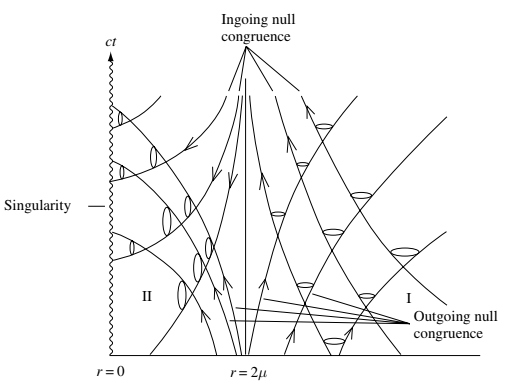
\includegraphics[width=0.7\textwidth]{Presentations/Images/4_bhphotons.png}
\end{figure}
\end{frame}

\begin{frame}{Radial photons and particles   worldlines in Schwarzschild coordinatesl}
\begin{itemize}
    \item On $(R_{\mathrm{I}})$: When $r\rightarrow \infty$ $\Rightarrow$ the metric tends to the Minkowski metric of special relativity and for $r\rightarrow 2\mu$ $\Rightarrow$ the coordinate $t$ follows that $t\rightarrow \pm\infty$.\\
    
    \item On $(R_{\mathrm{II}})$: Coordinates $t$ and $r$ reverse their character, then the lightcones flip their orientation by $90^{\circ}$. Furthermore, all photons must end up at $r=0$ and it follows that this point is a real singularity where the curvature of the Schwarzschild solution diverges.
\end{itemize}




\end{frame}

\section{Eddington-Finkelstein, Kruskal coordinates}
\begin{frame}{Eddington-Finkelstein coordinates}


A possible different set of coordinates is given by the null worldlines of radially moving photons. Using the integration constant on \ref{2} for both cases as the news coordinates, denoted by $p$, the coordinate transformation is given by 
 \begin{eqnarray}
 p= ct + r + Ln\Big| \frac{r}{2\mu}-1 \Big|\label{2}\\
 q= ct - r - Ln\Big| \frac{r}{2\mu}-1 \Big|\label{2}
 \end{eqnarray}
 Differentiating:
 \begin{eqnarray}
       dp&=&cdt +\frac{r}{r-2\mu}dr\\
       dq&=&
 \end{eqnarray}
 \begin{eqnarray}
  	ds^2 &=& \left( 1 - \frac{2\mu}{r}\right)dp^2-2dpdr- r^2 d\theta^2 - r^2 \sin^2 \theta d\phi^2\\
 	ds^2 &=& \left( 1 - \frac{2\mu}{r}\right)dq^2+2dqdr- r^2 d\theta^2 - r^2 \sin^2 \theta d\phi^2
 \end{eqnarray}
 
 
 
 
 
\end{frame}

\begin{frame}{Frame 1}

\end{frame}




\begin{frame}{Frame 1}

\end{frame}



\begin{frame}{Frame 1}

\end{frame}



\begin{frame}{Frame 1}

\end{frame}

\begin{frame}{Frame 1}

Para efectos de orden guardar imágenes como "4\_nombre.jpg/png/etc" en la carpeta "Images"

\begin{block}{Block 1}
\cite{hobson_efstathiou_lasenby_2006}    
\end{block}

\begin{figure}
    \centering
    
\includegraphics[width=0.25 \textwidth]{Presentations/Images/sample.jpg}
\end{figure}
    
\end{frame}

\end{document}